\documentclass{article}


\usepackage[utf8]{inputenc}
\usepackage{amsthm}
\usepackage{amssymb}
\usepackage{amsfonts}
\usepackage[francais]{babel}
\usepackage{fancyvrb}
\usepackage{hyperref}
\usepackage{graphicx}


\author{Ye Daniel, Kouadri Amine.} 

\title{Compte rendu du tp3}

\begin{document}

\maketitle
Ci-dessous les réponses aux questions du tp:

\paragraph{question 1.a:}
~~\\
\\ 
L'équation différentielle donnée est:
\\
$u'(x)= -u(x)$, $u(0)=1$
\\
on a $f(t,(u(t))=u'(t)=-u(t)$
\paragraph{question 1.c:}
~~\\
\\
la solution u est $u(t)= e^{-t}$
\\
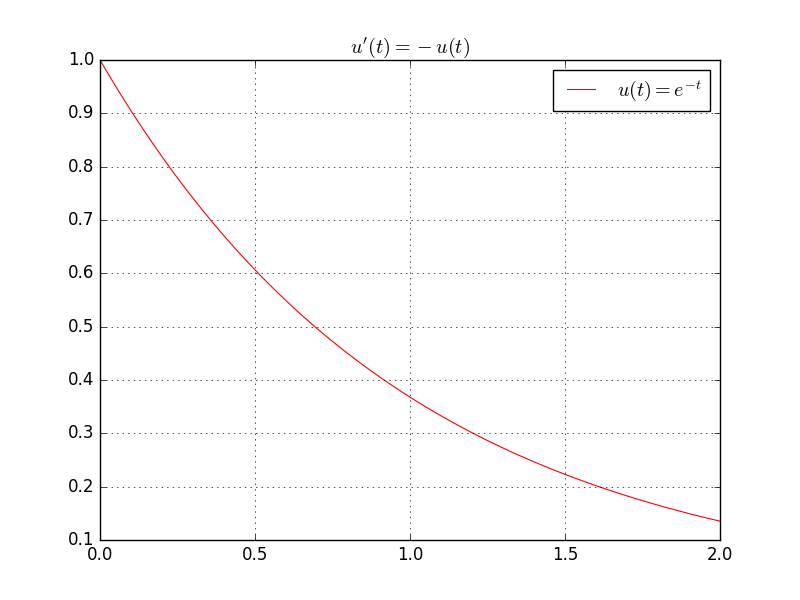
\includegraphics[height=5cm]{u1.png}

\paragraph{question 2:}
~~\\
\\
Méthode d'Euler:
Soit $u_{k+1}=u_k + h\times{f(t_k, u(t_k))}$
avec $f(t_k, u_k)=-u_k$ et $u_0=1.$
\\
h=T/n, On prend T=2 et n=10, on affiche à la console les valeurs de $u_{k+1}$:
\\
\\
$u_1\approx0.8
\\
u_2\approx0.64
\\
u_3\approx0.512
\\
u_4\approx0.4096
\\
u_5\approx0.32768
\\
u_6\approx0.26214400000000004
\\
u_7\approx0.20971520000000005
\\
u_8\approx0.16777216000000003
\\
u_9\approx 0.13421772800000004
\\
u_{10}\approx0.10737418240000003
\\
u_{11}\approx0.08589934592000002$

\paragraph{question 2.b:}
~~\\
\\
Représentation graphique de $u_k$ et des points ($t_k, u_k$).
\\
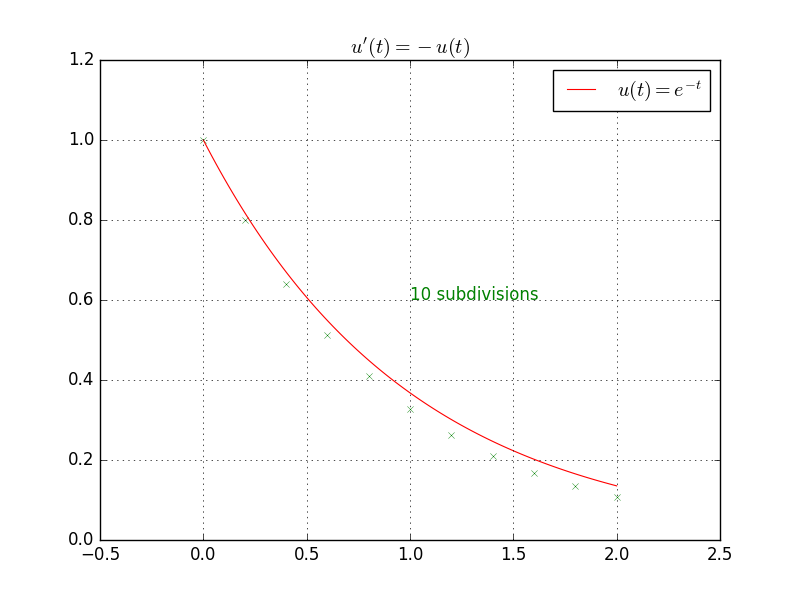
\includegraphics[height=8cm]{u1_10.png}

\paragraph{question 4.b:}
~~\\
\\
En appliquant la méthode Euler à l'exemple de la question 2 avec T=2 et n=30 on obtient le graphique suivant:
\\
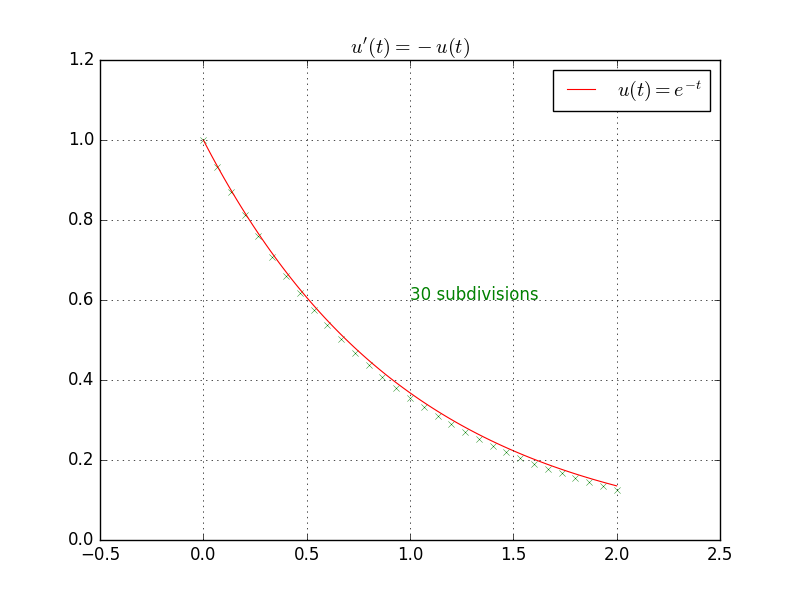
\includegraphics[height=8cm]{u1_30.png}
\\
\paragraph{question 4.c:}
~~\\
Voici les solutions des équations différentielles, on applique Euler à chacune de ces fonctions:
\\
$u'(t)=-u(t)+t$, $u(0)=1 \iff u(t)=2\times{e^{-t}+t-1}$
\\
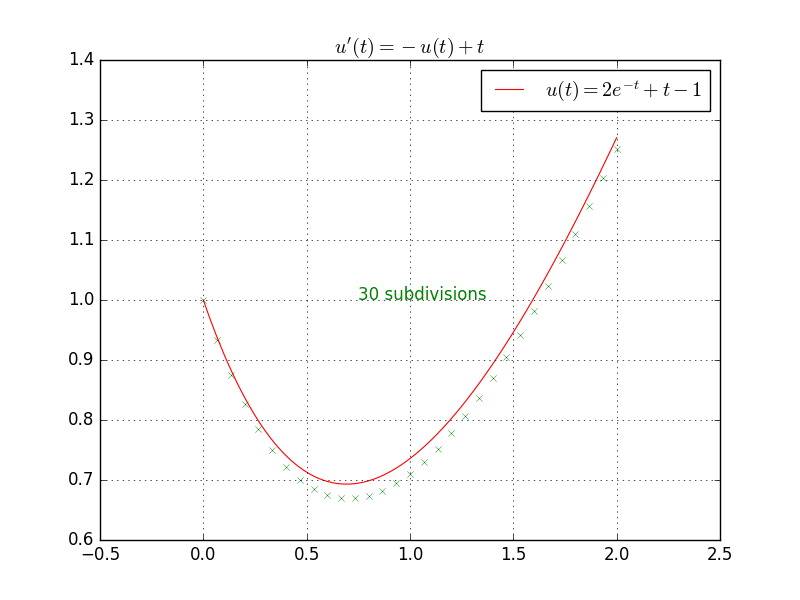
\includegraphics[height=8cm]{u2_30.png}
\\
$u'(t)= u(t)^2$, $u(0)=1 \iff u(t)=-\frac{1}{t-1}$
\\
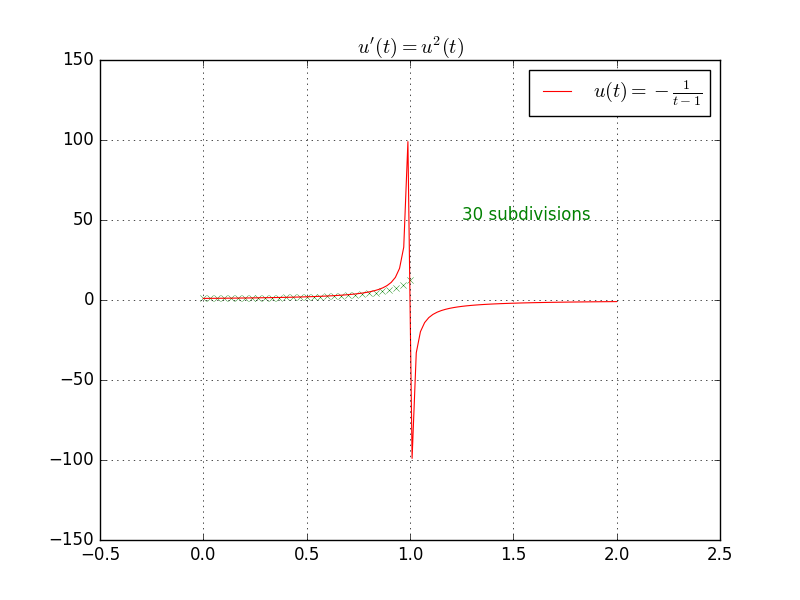
\includegraphics[height=8cm]{u3_30.png}
\\
$u'(t)=u(t)^2-t$
\\
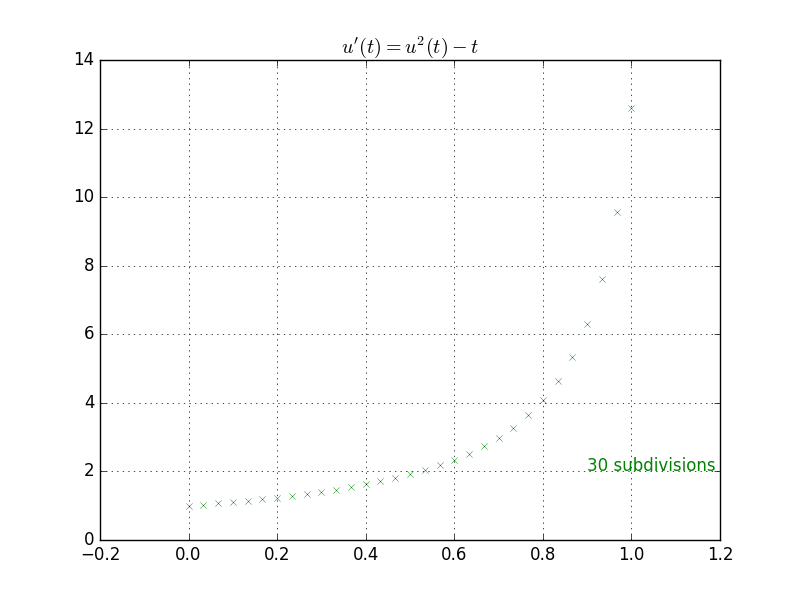
\includegraphics[height=8cm]{u4_30.png}
\\
\paragraph{question 5.1:}
~~\\
\\
La solution de l'EDO est : $u(t)=u_0\times{cos(\omega\times{t})}+\frac{v_0}{\omega}\times{sin(\omega\times{t})}$
\\
\paragraph{question 5.4:}
~~\\
\\
On prend $\omega=1$, $u(0)=1, v(0)=0$, et $T=4\pi$
on a donc $u(t)=cos(t)$
\paragraph{question 5.5:}
~~\\
\\
En appliquant la méthode d'Euler on obtient les graphiques suivants:
\\
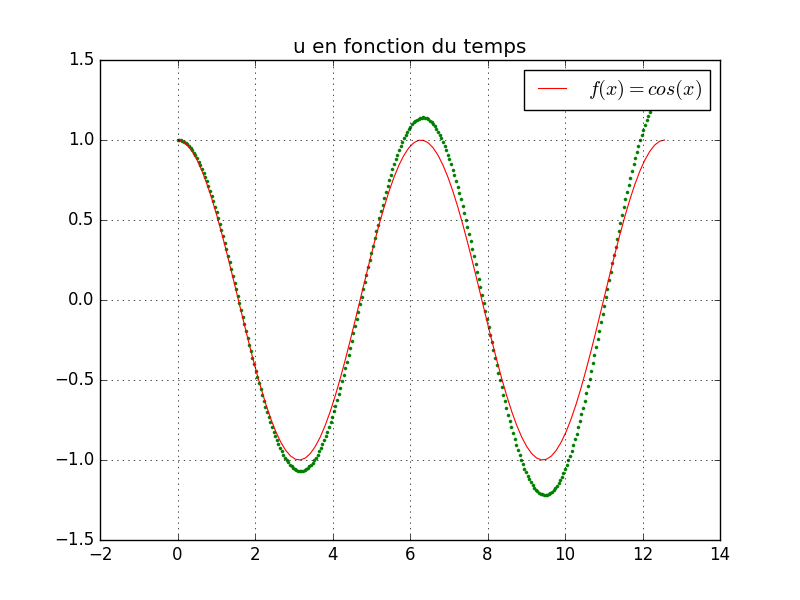
\includegraphics[height=8cm]{u_ft.png}
\\
\includegraphics[height=8cm]{v_ft.png}
\\
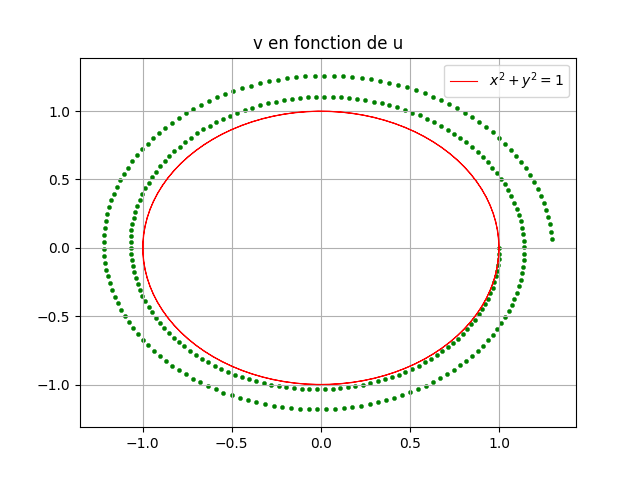
\includegraphics[height=8cm]{v_fu.png}
\\

\end{document}

